\documentclass{book}
\usepackage{graphicx}                              %for PNG images (pdflatex)
\usepackage[linkbordercolor={1.0 1.0 0.0}]{hyperref} %for \url tag
\usepackage{color}                                 %for defining custom colors
\usepackage{framed}                                %for shaded and framed paragraphs
\usepackage{textcomp}                              %for various symbols, e.g. Registered Mark
\usepackage{geometry}                              %for defining page size
\usepackage{longtable}                             %for breaking tables
%\usepackage{trackchanges}
%
\geometry{verbose,a4paper,tmargin=2.5cm,bmargin=2.5cm,lmargin=2.5cm,rmargin=2CM}
\hypersetup{
  pdfauthor = {},
  pdftitle = {Documentation of the Web Service based ARC Information System},
  pdfsubject = {},
  pdfkeywords = {Paper,keyword,comma-separated},
  pdfcreator = {PDFLaTeX with hyperref package},
  pdfproducer = {PDFLaTeX}
}
%
\bibliographystyle{IEEEtran}                       %a nice bibliography style
%
\def\efill{\hfill\nopagebreak}%
\hyphenation{Nordu-Grid}
\setlength{\parindent}{0cm}
\setlength{\FrameRule}{1pt}
\setlength{\FrameSep}{8pt}
\addtolength{\parskip}{5pt}
\renewcommand{\thefootnote}{\fnsymbol{footnote}}
\renewcommand{\arraystretch}{1.3}
\newcommand{\dothis}{\colorbox{shadecolor}}
\newcommand{\ngdl}{\url{http://ftp.nordugrid.org/download}~}
\definecolor{shadecolor}{rgb}{1,1,0.6}
\definecolor{salmon}{rgb}{1,0.9,1}
\definecolor{bordeaux}{rgb}{0.75,0.,0.}
\definecolor{cyan}{rgb}{0,1,1}
%
%----- DON'T CHANGE HEADER MATTER
\hyphenation{preserve-Original}
\begin{document}
\def\today{\number\day/\number\month/\number\year}

\begin{titlepage}

\begin{tabular}{rl}
\resizebox*{3cm}{!}{
\includegraphics{ng-logo.png}}
&\parbox[b]{2cm}{\textbf \it {\hspace*{-1.5cm}NORDUGRID\vspace*{0.5cm}}}
\end{tabular}

\hrulefill

%-------- Change this to NORDUGRID-XXXXXXX-NN

{\raggedleft NORDUGRID-TECH-21\par}

{\raggedleft \today\par}

\vspace*{2cm}

%%%%---- The title ----
{\centering \textsc{\Large ARC Information System}\Large \par}
\vspace*{0.5cm}
    
%%%%---- A subtitle, if necessary ----
{\centering \textit{\large Documentation and developer's guide}\large \par}
    
\vspace*{1.5cm}
%%%%---- A list of authors ----
    {\centering \large \footnote{@} \large \par}
\end{titlepage}

\tableofcontents                          %Comment if use article style
\newpage

\renewcommand{\thefootnote}{\arabic{footnote}}


\chapter{Design Overview}
\label{cha:design_overview}

\begin{figure}[ht]
 \centering{
  \scalebox{0.6}{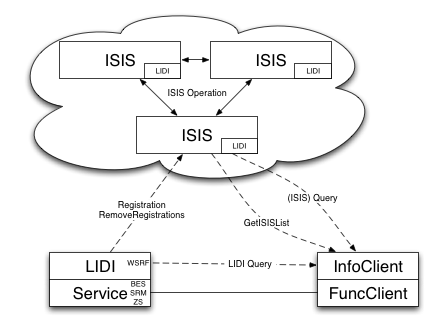
\includegraphics{SystemOverview.png}}
  \caption{\label{fig:infosys_architecture}Architecture of Information System}
 }
\end{figure}

Information System of ARC middleware is composed of 3 main parts. The Information System Indexing Services (ISIS) form a set of information containers. Every generic ARC Service pushes information about itself into nearby ISIS container/service hence registering itself to Information System. The information stored in every ISIS is propagated among all ISIS services. Clients can query any nearby ISIS service for registered information in order to perform discovery of services which posses specific properties. Clients can also query ARC Services to obtain more detailed information about Service properties.

\chapter{ISIS}
\label{cha:isis}

\section{Registration handling}
\label{sec:isis_registration_handling}

\subsection{Functionality}
\label{sub:isis_functionality}

 The functionality of ISIS is made of two parts. On the one hand they are working as ordinary Web Services, and on the other hand maintain a peer-to-peer network - \texttt{ISIS cloud}.

 Main functionality of ISIS service visible from outside of ISIS cloud is to accept registration and provide collected information to clients. For that ISIS implements operations described in following section.
The single ISIS service accepts Registration Records pushed to it by other services (including ISIS services too) and stores them in local XML database. Stored records can be queried by clients using mandatory and service-specific attributes for selection criteria.

 In case of multiple ISIS services they form a peer-to-peer network. Inside that cloud Registration Records are propagated between services in such a way that all ISIS instances continuously try to synchronize their databases.

% TODO: put figure here

% subsection functionality (end)

\subsection{Interface} 
\label{sub:isis_interface}

\subsubsection{Operation Register}

\begin{description}

  \item[Input]~\begin{description}
    \item[Header]~\begin{description}
      \item[RequesterID] Identifier of the client.
      \item[MessageGenerationTime] Time when following set of RegEntry was generated. There may be multiple RegEntry elements.
    \end{description}
    \item[RegEntry]~\begin{description}
      \item[SrcAdv]~\begin{description}
        \item[Type] Type of service being registered. This element is opaque string for now. There shall be service types defined later.
        \item[EPR] Endpoint Reference of service being registered in terms of WS-Addressing.
        \item[SSPair] Set of key/value pairs representing service specific information.
      \end{description}
      \item[MetaSrcAdv]~\begin{description}
        \item[ServiceID] Globally unique and persistent identifier of the service.
        \item[GenTime] (Generation Time) The actual timestamp of information (called wake\_up\_time in the pseudo code below)
        \item[Expiration] Validity period of Service Advertisement record.
      \end{description}
    \end{description}
  \end{description}

  \item[Output]~\begin{description}
    \item[Fault] Optional element describing fault which occurred while performing registration. If missing registration succeeded.
  \end{description}

  \item[Faults]~\begin{description}
    \item[none]No specific faults are defined
  \end{description}

\end{description}

This operation is usually called by service which wants to register it's presence in ISIS. This message consists of one or more \textbf{Registration Entry} and at most one \textbf{Registration Header}. The \textbf{Registration Entry}(RegEntry) contains a \textbf{Service Advertisement}(SrcAdv) and a corresponding \textbf{Service Advertisement Metadata}(MetaSrcAdv). This structure is shown on Figure \ref{fig:registration_message}.
\begin{figure}[ht]
\centering{{\scalebox{0.6}{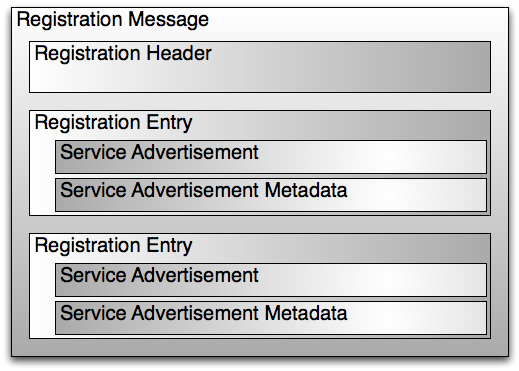
\includegraphics{RegistrationMessage.png}}}
\caption{\label{fig:registration_message}Embedded structure of Registration Message} }
\end{figure}

Service must supply mandatory information. Among those the \texttt{Endpoint Reference} is used to contact service - only required element is contact URL of service. \texttt{Type} specifies kind of service and is used to find out functionality and interface of service. \texttt{ServiceID} is used to distinguish between registered services and to deal with case of service changing it's contact URL. For more information about mandatory and optional information see Section \ref{service_advertisement}

As result of this operation new Registration Record is stored inside ISIS internal database and eventually propagated to other ISISes. If registration record of same ID already existed it will be renewed.

This operation is also used by ISIS services to propagate Registration Records inside ISIS cloud.

\subsubsection{Operation RemoveRegistrations}

\begin{description}

  \item[Input]~\begin{description}
    \item[MessageGenerationtime]
    \item[ServiceID] Multiple identifiers of services, whose records has to be removed.
  \end{description}

  \item[Output]~\begin{description}
    \item[RemoveRegistrationResponseElement]~\begin{description}
      \item[ServiceID] Identifier of service whose record was not removed
      \item[Fault] Description of failure reason
    \end{description}
  \end{description}

  \item[Faults]~\begin{description}
    \item[none]No specific faults are defined
  \end{description}

\end{description}

This operation is used to explicitly requesting the removal of zero or more Registration Entries associated with specified ServiceID values stored in the Information System. If corresponding record does not exist it's identifier will be present in response message together with corresponding Fault element.

\subsubsection{Operation GetISISList}

\begin{description}

  \item[Input]~\begin{description}
    \item[none]
  \end{description}

  \item[Output]~\begin{description}
    \item[EPR] Multiple Endpoint References of known ISIS services
  \end{description}

  \item[Faults]~\begin{description}
    \item[none]No specific faults are defined
  \end{description}

\end{description}

In response to this operation the EndpointReferences to all known ISIS services are returned. The operation is used for obtaining a list of known ISIS instances from any particular ISIS. Clients can then use the obtained list to run direct queries against the ISIS instances. The operation is provided for fault tolerance and for providing optional performance boost. This operation returns the known peer-to-peer neighbors. If client is interested in all ISIS instances they can be obtained using the Query operation because they are ordinary services registered into the Information System.

\subsubsection{Operation Query}

\begin{description}

  \item[Input]~\begin{description}
    \item[QueryString] XPath query expression
  \end{description}

  \item[Output]~\begin{description}
    \item[any] Result of query
  \end{description}

  \item[Faults]~\begin{description}
    \item[none]No specific faults are defined
  \end{description}

\end{description}

This operation allows any XPath queries to be performed on stored Registration Records. The records are treated as merged in one XML document with each record being equivalent to \texttt{RegEntry} element of \texttt{Register} operation. In response all elements produced by XPath query are returned. The purpose of this operation is to make it possible to obtain any kind of information related to the Indexing Database.

% subsection interface (end)

% section registration_handling (end)

\section{Peer-to-Peer}
\label{sec:isis_peer_to_peer}

\subsection{Functionality}
\label{sub:peer_to_peer_functionality}
The ISISs are able to organize themselves into a peer-to-peer network by synchronizing the stored replicated database and maintain this synchronicity and network topology. Every node of this peer-to-peer cloud (that�s an ISIS service) has an own PeerID (an identifier only used in this network) made as a hash of its endpoint URL. The members are ordered by this identifier where there is also a sequence defined between them where the follower of the entity is the ISIS with the smallest PeerID of the greater PeerIDs and the smallest in case of the greatest value. This metric is used for define the neighbor relation that�s the base of the inter-peer-to-peer network communication. A strong condition that only registered ISIS can have any role in the cloud.

\subsubsection{Connecting to the peer-to-peer network}
Every ISIS tries to connect to the network at its startup by accessing the InfoProvider ISISs  known from the configuration. The order of attempting is random to achieve as much load-balancing as possible. (By design we are counting of a huge amount of ISISs configured in a very similar way, where the InfoProvider ISIS are mainly the same.) If there is no InfoProvider available or nothing is known from the configuration, the node decides to be the fist member and to build a new network.

If there is any InfoProvider available the list of member ISIS will be queried and the �follower� will be defined using the previously mentioned metric. This �follower� node will help the ISIS to connect to the cloud. The new member will use the �Connect� Web Service operation to get the newest version of database stored in the peer-to-peer network, and place the newer entries to the cloud by register them. An initial database synchronization can be achieved with this process.

We can prevent to overload the InfoProvider ISISs by balancing the operation of database synchronizing that�s the most costly procedure in the connection phase.

There is also an other extension used in connection with the InfoProvider ISISs. If a node wasn't able to connect any of its InfoProviders then it will redo that later. This achieves that the network is able to fuse two disjunct parts of network when the missing InfoProvider ISIS is appearing.

\subsubsection{Routing in the peer-to-peer network}
We are keeping the databases in synch by passing every Registration and RemoveRegistrations  to every node acting in the network. This set the redundancy and the fault tolerant message routing very important between any two ISISs.

The most important parameter of the network is the {\it sparsity}. This an integer not less then 2 that determines the number of neighbors in the function of the actual number of member nodes of the network, where the number of neighbors can be growing when new members connecting to the network or members leave. A spares graph can be shaped by choosing a great value to sparsity or a dense by choosing the most less. This value is defined during the design and determines the main properties of the peer-to-peer network.
\begin{figure}[ht]
\centering{{\scalebox{0.6}{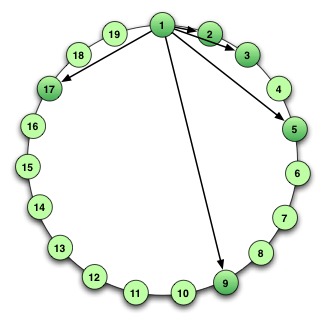
\includegraphics{Circle2-1.png}}}
\caption{\label{fig:p2p_neighbors_2} The neighbor connections in the peer-to-peer network in case of sparsity=2} }
\end{figure}

Every node has always exactly n = $\lceil \log_s{N} \rceil$ neighbors where the $N$ is the number of the ISIS registered into the network. The node has as neighbor the ISISs with PeerID $s^0$-th, $s^1$-th ... $s^{n-1}$-th greater than the own. (For example: There is 19 nodes in a network with sparsity=9. Then the 1st node has as neighbors the 2nd, 3rd, 5th, 9th, and 17th node as seen on figure \ref{fig:p2p_neighbors_2}.)

There can be exactly n redundancy achieved in the system so at most $n-1$ node can be disappear without any serious communication problem. Since we are also using a method that tries to deliver the message even every neighbor is unavailable, this fault tolerance is much greater. With this extension, we will pass the message to at least one other available ISIS so the message wont stick if the node is not the only working node in the network. This solution provides a secure and quite fast solution for the message deliver but has a high communication cost because there is $n*N$ message necessary in general for every Registration or RemoveRegistrations.

If there is a much greater {\it sparsity} used that's even greater then the number of the expected number of members then every node will have only one neighbor. This situation can be seen on Figure \ref{fig:p2p_neighbors_40}. In this case it can be such a functioning achieved where is only N (the theoretically minimum) message in the network at the expense of a slower propagation.
\begin{figure}[ht]
\centering{{\scalebox{0.6}{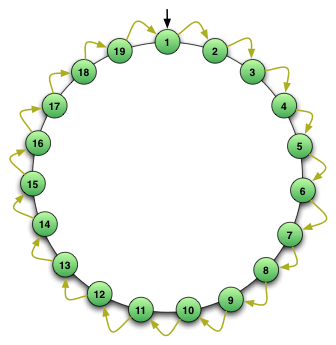
\includegraphics{Circle40-40.png}}}
\caption{\label{fig:p2p_neighbors_40} The neighbor connections in the peer-to-peer network in case of sparsity>N} }
\end{figure}

There is a data-driven routing used in the peer-to-peer cloud. It means that the given nodes examines the received Registration Entries and store and forward only the newer ones than the already known version belonging to the same service identifier. If the information is out-of-date then it will be simple dropped. (A Coordinated Universal Time (UTC) standard time and date format is used for the time stamps that is also able to handle the differences originated from the different time zones.) We managed to achieve using this method not to store the already deliver nodes list in the message but deciding about the forwarding locally based on locally available information. Since the routing is based on time stamps, it is very important to keep the nodes clock in synch with each other or with an outer reference for example by using NTP.

An other advantage of this solution is the ability of handling the case of medley Register and RemoveRegistrations messages. It is possible for a RemoveRegistrations message to forerun a previously generated Register message. This cause just a temporary imprecise entry in the database but the mistake can be quickly fixed and won't be much further propagated.

Since we are base our routing to the state of the messages belonging to the service identifier it is important to keep the fact of message deleting for a while. If we are receiving a RemoveRegistrations message then do not remove the named entry from the database just change its state to {\it deleted} by keeping only a piece of data about it (the service identifier and the deletion time). 

\subsubsection{Maintenance of the peer-to-peer network}
In the network there is two different maintenance needed. On the one hand the database have to be periodically kept up and on the other hand the list of neighbors have always to be up-to-date.

The database applied in the system is a soft-state database so the entries are {\it valid} just for a limited time. Without any registration freshening it's validity will expire and the entry's state will change to {\it expired}. The time of expiration have to be defined to every singe message by the registrar entity. The RemoveRegistrations message turn the state of registration entry {\it deleted} as it was previously mentioned. The {\it expired} or {\it deleted} messages will purged for good and all in the course of the periodical database maintenance. The states of registration entries can be shown on Figure \ref{fig:RegEntry states}.
\begin{figure}[ht]
\centering{{\scalebox{0.6}{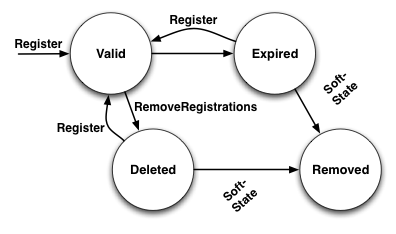
\includegraphics{RegEntryStates.png}}}
\caption{\label{fig:RegEntry states} Registration entry states} }
\end{figure}

The second kind of maintenance is keeping the list of neighbors up-to-date. While receiving even Registration or RemoveRegistrations messages or found an outdated entry during the periodical database cleaning we are doing the necessary steps to update our list. Since every leaving or entering node has influence to the every node's neighbor registry with a high probability it will be rebuilt in these cases. The modification are passing locally because this connections are asymmetric so there is no compliance or network communication is needed.

There is no special action done and no additional network traffic needed during the neighbor checking. The fact the node sends periodically messages to every neighbor can be exploited. If the node do not success to send its message to the neighbor after some tries, then the unavailable node will be marked. If every neighbor will be getting marked then the node change its PeerID and reconnect to the network if any InfoProvider ISIS is available.

When a neighbor is unavailable we keep also trying to deliver the message to the followers of the neighbor until we manged to find one to pass the information or diagnose that every nodes are unavailable. Here the follower means the nodes that have greater PeerID than the neighbor has but less then our next neighbor. 
% subsection functionality (end)

\subsection{Interface}
\label{sub:isis_peer_to_peer_interface}
\subsubsection{Operation Connect}

\begin{description}

  \item[Input]~\begin{description}
    \item[none]
  \end{description}

  \item[Output]~\begin{description}
    \item[RegEntry] Multiple \texttt{RegEntries} locally stored in the ISIS database
  \end{description}

  \item[Faults]~\begin{description}
    \item[none]No specific faults are defined
  \end{description}

\end{description}

This operation allows the ISIS to get the already existing database from the ISIS that helps it to connect the peer-to-peer network. As a second step of the connection the newer  \texttt{RegEntries} that are stored at the connecting entity will be propagated through \texttt{Register} operation of the standard service specific interface.

% subsection interface (end)

% section peer_to_peer (end)

\section{Authorization}
\label{sec:isis_authorization}

\subsection{Client Authorization}
\label{sub:isis_authorization_client_authorization}

% TODO figure with mutiple service types

\textit{This section extensively uses terms defined in "Security Framework of ARC1" document"~\cite{arcsec}.}

To ensure information stored in ISIS cloud can't be tampered and only available to proper clients following authorization framework is implemented. All actions performed by ISIS clients are divided into three following groups:

\begin{itemize}
 \item Operations initiated by other ISISes in the cloud. Those include:
 \begin{itemize}
  \item Register with Registration Message containing information not about contacting client
  \item RemoveRegistrations with request to remove Registration Message representing not contacting client
  \item Connect indicating to provide every information about the stored database
 \end{itemize}

 Those operations may cause uncontrollable changes in collected information and must be granted only for highly trusted entities like ISISes themselves.

 \item Operations initiated by the Services registering to Information System. Those are:
 \begin{itemize}
  \item Register with Registration Message containing information about contacting client
  \item RemoveRegistrations with request to remove Registration Message representing contacting client
 \end{itemize}

 \item Operations which are allowed for any liable client of particular Grid infrastructure.
 \begin{itemize}
  \item Query
  \item GetISISList
 \end{itemize}
\end{itemize}

Those 3 action groups are handled using Security Framework of ARC~\cite{arcsec}. For each group corresponding 
Action is defined for ARC policy language as described in table \ref{tab:policy_actions}.

\begin{table}[h]
\caption{ARC Policy Actions of ISIS}
\label{tab:policy_actions}
\begin{tabular}{|c|c|l|}
\hline
\textbf{Group}&\textbf{Action}&\textbf{AttributeId}\\
\hline
Request from ISIS&\textit{isis}&http://www.nordugrid.org/schemas/policy-arc/types/isis/operation\\
\hline
Request from Service&\textit{service}&http://www.nordugrid.org/schemas/policy-arc/types/isis/operation\\
\hline
Request from generic client&\textit{client}&http://www.nordugrid.org/schemas/policy-arc/types/isis/operation\\
\hline
\end{tabular}
\end{table}

Access restrictions for clients are defined using ARC Policies which are specified and 
processed using generic Security Handlers approach. Corresponding Security Handlers have to be 
configured inside configuration block of corresponding ISIS service and attached 
\textit{incoming} queue.

% subsection client_authorization (end)


\subsection{Information Authorization}
\label{sub:isis_authorization_information_authorization}

Because all ISIS services trust each other they freely exchanging collected information. But 
not all information stored inside ISIS cloud is public or readable by clients authorized according 
to procedure described in section \ref{sub:isis_authorization_client_authorization}. There
may be some pieces of information available only for specific clients. An example could be 
information about resources serving particular Virtual Organization (VO) could be visible only to
members of that VO.

To implement functionality described above each node in aggregated XML documents of information
collected by ISIS cloud may have Access Control Policy associated with it. Access control is 
defined at level of XML node and propagates all children nodes - similar to file systems.
Children nodes can only additionally restrict access control imposed by parent node. For example
if parent node A allows access only to VO1 then children node B can narrow access to Administrator 
of VO1 and can't grant access for VO2 members.

By default all XML nodes are public. Access Control Policies are embedded into XML document
as XML nodes (see Appendix \ref{annex:info_policies_schema} for schema) even if that violates schema 
of document. Then nodes are assigned policies by adding XML attributes referring to defined Policies.
Access permission to particular information node is evaluated by traversing all nodes prom 
parent to children. At first node which gives negative result evaluation is stopped and
this node including all its children is removed from document.

Before providing results of query operation ISIS runs procedure described above on results and 
also removes Access Control Policies. Reduced document obtained in this way is returned to
requesting client.

%* Clasification of information
%
% 1. From acccessibility point of view information can be devided
%into 3 groups:
% a. public
% b. available to trusted clients (like broker or scheduler service)
% c. private - available to owner of information object and entities
%trusted by owner.
%Distinction between 2 and 3 is not clear. One may accept that 2 is
%imposed by architecture/deployment of system and 3 is controlled by
%entities which are users of the system.
% 2. From storage/access location point of view information is divided
%into:
% a. local - stored at endpoint representing resource which is
%described by information. This information is obtainable through
%ALIS interface.
% b. propagated to dedicated services (ISIS) which collect information
%needed for pre-selection and initial lookup of services
%representing resources.
%
%NOTE: Definition of propagation of information does not exactly belong
%to security architectire of information system. But it affects it significantly
%and hence at least minimal set of definitions is needed.
%
%OUT OF BAND NOTE: Those services could provide pre-selection capability.
%
% Sets 1 and 2 may intersect in any way. In first approach to simplify
%implementation 2b may be considered to always belong to 1a.
%
%
%* Implementaion guidelines
%
% To implement set 1 information objects need to have Access Control
%Rules (ACR) assigned (usually used term Access Control List seems to
%be inadequate due to meaning of word List).
%
% To implement set 2 in similar way information objects have Propagation
%Control Rules (PCR) assigned. Because curently information system is made
%of one layer of ISIS PCRs may consist of one boolean property.
%
% Information is structured in tree-like fashion - XML document.
%Access control is defined at node and follows all branches - similar
%to file systems. Propagation control is similar to access control (if
%needed at all). Children nodes can't widen access defined at parent
%nodes. This should decrease amount of ACR to be evaluated.
%
%EXAMPLE: if parent node A allows access only to VO_1 then children
%node B can narrow access to Adminsitrator of VO_1 and can't open
%access for VO_2.
%
% By default all nodes are public and are propagatable. Properties
%assigned to clildren nodes limit access and propagation. Access
%permission to particular information node is evaluated by traversing
%all nodes prom parent to child. At first node which gives negative
%result evaluation is stopped.
%
% Because evaluation of permission may be costly (CPU intensive,
%causing big latency if access to external service is needed, etc.)
%other tricks to reduce cost are needed.
%
% To reduce access control evaluation cost ACRs may/should/must(?)
%be assigned to information nodes in one-to-many way - one ACR per
%multiple information nodes. This grouping may be initiated either
%interactively (by clients explicitely specifying that same ACR is
%applicable to multiple nodes) or automatically (by comapring new
%ACR to already existing).
%
% If information nodes containing ACRs are propagated to ISIS (second
%implementation step) propagation algorithm must take ACR into account.
%For informtion propagation between ISISes this rule also applies.
%EXAMPLE: Information with access open to VO_1 must not be propagated
%to ISIS belonging to VO_2.
%
%
%** Ideas for in-memory XML documents
%
% Because informational documents are normally produced dynamically and
%have short lifetime there seems to be reasonable to keep them in memory.
% Each node with assigned ACR contains attribute (even if that breaks schema)
%containing id of ACR. ACR is defined as XML element (even if that breaks
%schema) located at higher, same or child level of considered node.
% Because informational documents are produced dynamically there are few
%ways for processing ACRs:
% 1. Right after document is generated it is traversed and ACRs applied.
%Parts of document which do not pass ACR evaluation are cut off. ACRs are
%cut off too.
% 2. While calling document generation procedure identity of client is
%supplied and ACRs are applied immediately.
% 3. While calling document generation procedure hooks/callbacks are supplied
%which are used and implement ACR evaluation.
% Combination of 1 and 3 looks most promising because it is flexible and
%keeps information system and policy evaluation code separated.
%
%
%* References
%"Information access control use cases" http://wiki.nordugrid.org/index.php/ARC1/Infosys/Access_Use_cases
%

% subsection information_authorization (end)

\subsection{Configuration}
\label{sub:isis_authorization_configuration}

\textit{For information about sophisticated authorization policies and how to deploy various Policy Decision Point entities please see "Security Framework of ARC1" document"~\cite{arcsec}.}

To restrict set of clients allowed to perform operations in ISIS service proper authorization policy is needed. Let's assume ISIS is operating over TLS connection and all participants posses X.509 certificates with following subject names:
\begin{itemize}
\item /O=Grid/O=Test/CN=CLIENT - generic client entities
\item /O=Grid/O=Test/CN=SERVICE - generic service entities
\item /O=Grid/O=Test/CN=ISIS - all ISIS belonging to ISIS cloud
\end{itemize}

\textit{In NO way we suggest to use such setup. Real installation should use more sophisticated way to 
identify clients contacting ISIS service. For an infrastructure with quite static roles distribution for 
example we suggest to use Virtual Organization Management Service (VOMS) attributes embedded into X.509 
certificates representing participating entities.}

Below is an example policy made of 3 rules defined in lines 4-17, 18-29 and 30-39. Those define allowed 
behavior for ISIS, generic service and generic client. Lines 6-7, 20-21 and 32-33 specify attributes 
used to recognise type of connecting client. In this case those are subjects of X.509 certificates with 
values defined above. Lines 10-15, 24-27 and 36-37 specify allowed actions. One can see that this policy 
allows all operations to be performed by ISIS client. It limits operations allowed for generic service 
to "service" and "client" types. And client entities are allowed to perform "client" type operations only.

\begin{verbatim}
 1: <?xml version="1.0" encoding="UTF-8"?>
 2: <Policy xmlns="http://www.nordugrid.org/schemas/policy-arc" PolicyId="policy1"
 3:           CombiningAlg="Deny-Overrides">
 4:  <Rule RuleId="isis_to_isis" Effect="Permit">
 5:    <Subjects>
 6:      <Subject AttributeId="http://www.nordugrid.org/schemas/policy-arc/types/tls/identity"
 7:              >/O=Grid/O=Test/CN=ISIS</Subject>
 8:    </Subjects>
 9:    <Actions>
10:      <Action AttributeId="http://www.nordugrid.org/schemas/policy-arc/types/isis/operation"
11:             >isis</Action>
12:      <Action AttributeId="http://www.nordugrid.org/schemas/policy-arc/types/isis/operation"
13:             >service</Action>
14:      <Action AttributeId="http://www.nordugrid.org/schemas/policy-arc/types/isis/operation"
15:             >client</Action>
16:    </Actions>
17:  </Rule>
18:  <Rule RuleId="service_to_isis" Effect="Permit">
19:    <Subjects>
20:      <Subject AttributeId="http://www.nordugrid.org/schemas/policy-arc/types/tls/identity"
21:              >/O=Grid/O=Test/CN=SERVICE</Subject>
22:    </Subjects>
23:    <Actions>
24:      <Action AttributeId="http://www.nordugrid.org/schemas/policy-arc/types/isis/operation"
25:             >service</Action>
26:      <Action AttributeId="http://www.nordugrid.org/schemas/policy-arc/types/isis/operation"
27:             >client</Action>
28:    </Actions>
29:  </Rule>
30:  <Rule RuleId="client_to_isis" Effect="Permit">
31:    <Subjects>
32:      <Subject AttributeId="http://www.nordugrid.org/schemas/policy-arc/types/tls/identity"
33:              >/O=Grid/O=Test/CN=CLIENT</Subject>
34:    </Subjects>
35:    <Actions>
36:      <Action AttributeId="http://www.nordugrid.org/schemas/policy-arc/types/isis/operation"
37:             >client</Action>
38:    </Actions>
39:  </Rule>
40: </Policy>

\end{verbatim}

This policy is not as restrictive as it could be in order to allow ISIS register themselves as ordinary 
services and to allow services which perform discovery of other services to behave like ordinary clients.

In order to activate policy it must be linked to ISIS service through Security Handle and Policy 
Decision Point emedded into configuration of ISIS. Below is minimal example configuration element of 
ISIS service. In lines 7-17 a set of Security Handler and Policy Decision Point is configured to handle
policies written in ARC Policy Language (described in ~\cite{arcsec}). Line 14 specifies that policy is 
read from file \textit{/opt/arc/etc/isis/policy.xml} every time new request is arrived. If policy is not 
satisfied then ISIS returns SOAP Fault instead of usual informative response.

\begin{verbatim}
 1: <Service 
 2:   xmlns="http://www.nordugrid.org/schemas/ArcConfig/2007"
 3:   xmlns:isis="http://www.nordugrid.org/schemas/ArcConfig/2009/isis"
 4:   name="isis" id="isis">
 5:  <isis:endpoint>https://localhost:60000/isis</isis:endpoint>
 6:  <isis:DBPath>/opt/arc/share/isisdb</isis:DBPath>
 7:  <SecHandler
 8:    xmlsns:auth="http://www.nordugrid.org/schemas/SimpleListAuthZ"
 9:    name="arc.authz" id="authz" event="incoming">
10:   <auth:PDP
11:     xmlns:pdp="http://www.nordugrid.org/schemas/ArcPDP"
12:     name="arc.pdp">
13:    <pdp:PolicyStore>
14:     <pdp:Location type="file">/opt/arc/etc/isis/policy.xml</pdp:Location>
15:    </pdp:PolicyStore>
16:   </auth:PDP>
17:  </SecHandler>
18: </Service>

\end{verbatim}

% subsection information_authorization (end)


% section authorization (end)

% chapter isis (end)

\chapter{Service}
\label{cha:service}

\section{Information generation}
\label{sec:service_information_generation}

The service developers have to ensure that the services are providing the necessary information about 
themselves when registering to ISISes. This is done by implementing the subclass of the Arc::Service class - 
the RegistrationCollector function has to provide up-to-date status information about the service and anything 
else it wants to be advertised. This information package is called \textbf{Service Advertisement}.
\label{service_advertisement}
The \textbf{Service Advertisement} can contain any information service wants to advertise but the mandatory 
elements have to be always present:
\begin{itemize}
  \item Service ID: A globally unique identifier of the service.
  \item Service Type: The Glue2 type of service.
  \item Endpoint URL: The URL where the service can be contacted provided as part of EPR element.
\end{itemize}

Because there may be multiple registration processes running in parallel it is important to ensure that 
implementation of RegistrationCollector is thread safe or there are internal locks implemented.

Every service registering to ISIS should also provide an interface for direct querying of information 
describing service. Normally this information should be more detailed than one sent to ISIS. For this 
purpose LIDI interface is defined which is a subset of WS Resource Properties (WSRP)~\cite{wsrf-rp}. Following WSRP
operations must be supported - \textit{GetResourcePropertDocument}, \textit{GetResourceProperty},
\textit{GetMultipleResourceProperties} and \textit{QueryResourceProperties}.

%TODO: define names of mandatory properties - at least Glue2 property


% section information (end)

\section{Registration}
\label{sec:service_registration}

The registration of service is carried out by internal module called Registrant. The Registrant is active module of the HED (Hosting Environment Daemon) which is bound to a set of ISISes. In practice, the configuration part of the Registrant contains exactly one ISIS to bind, and the Registrant will collect the necessary information about the other ISISes belonging to the same network.

To register services to more than one ISIS network multiple Registrant instances has to be configured. In this case, the default Registrant will be used for registering every services unless configured explicitly.
The registration of service can be done once or periodically based either on the configuration of the Registrant or overwritten for every service separately. The Registrant is also performing message aggregation of all services linked to it if possible. The simplified algorithm of the Registrant is presented below.

\begin{framed}
  Registrant - pseudo algorithm\\
  \\
  \verb#// Initialize phase#\\
  \verb#Read the configuration and store the information about the services in a list#\\
  \verb#do { // Cyclic phase in a different Thread#\\
  \verb# wake_up_time = now();#\\
  \verb# messages = null;#\\
  \verb#  if ( 0 < count(service where service.next_run <= wake_up_time)) {#\\
  \verb#    foreach( service where service.next_run <= wake_up_time) {#\\
  \verb#      messages.add(service.RegistrationCollector);#\\
  \verb#      service.next_run = wake_up_time + service.period;#\\
  \verb#    }#\\
  \verb#    if (0 < count(messages)) {#\\
  \verb#      sent_message = assemble message with headers(messages);#\\
  \verb#      send(sent_message);#\\
  \verb#    }#\\
  \verb#  } else {#\\
  \verb#    sleep(min(service.next_run) - now()); #\\
  \verb#  }#\\
  \verb#} while(true)#\\
\end{framed}
Current implementation does not allow value of the period to be less than 2 minutes.

Service provides \textbf{Service Advertisement} part of information sent to ISIS (see Section \ref{sub:isis_interface}).
Before sending this information the Registrant extends it with additional data (\textbf{Service Advertisement Metadata}).

An example layout of services is shown on Figure \ref{fig:registration_overview}. In this configuration example 
there are two Registrants configured in one HED container for three services. The \textit{Registrant A} is the 
default Registrant and the services configured in the following way:

\begin{itemize}
  \item Service 1: There is no Registrant configured so the default one will register it.
  \item Service 2: The \textit{Registrant A} is configured explicitly.
  \item Service 3: The \textit{Registrant B} is configured explicitly.
\end{itemize}

So the Service 1 and 2 are handled both by \textit{Registrant A} and Service 3 by \textit{Registrant B}.
In the first step each Registrant performs information collection from all assigned services sequentially. Registrants themselves are executing in parallel. For Figure \ref{fig:registration_overview} the approximate sequence of information collection is (\textit{A1}-\textit{A2}, \textit{B1}-\textit{B2}) followed by (\textit{A3}, \textit{A4}). After collection  the aggregated information is sent to the corresponding ISISes independently by each other Registrant (\textit{A5}, \textit{B5}).

\begin{figure}[ht]
\centering{{\scalebox{0.6}{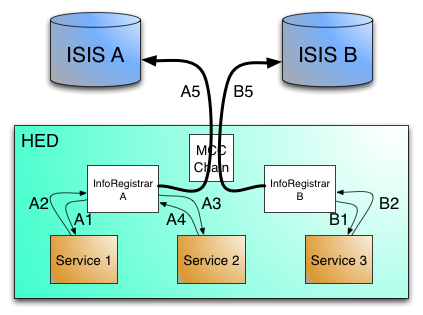
\includegraphics{Registration.png}}}
\caption{\label{fig:registration_overview}Overview of the registration process} }
\end{figure}

This registration operation is done once during the start-up phase and periodically according to 
(per service) configured periods.

% section registration (end)


\section{Authorization}
\label{sec:service_authorization}

For each information provided by service through the LIDI interface same procedure as described in 
Section \ref{sub:isis_authorization_information_authorization} should be applied.

% section authorization (end)


\section{Configuration}
\label{sec:service_configuration}

The registration operation is done by the Registrants as described in Section \ref{sec:service_registration}.
Each Registrant is instantiated by corresponding InfoRegistrar XML element in configuration file as 
defined in Section \ref{annex:service_configuration_schema}. First InfoRegistrar defines Registrant 
which is used to register every service by default.

Registration parameters per service are defined by InfoRegister element located inside corresponding 
service configuration element. To assign service to specific Registrant(s) one may use Registrar 
configuration elements situated inside InfoRegister. If none Registrar element is defined service will 
be registered using first (default) Registrant. To make not register itself special configuration element 
NoRegister has to be used.

Following elements are defined inside configuration element of the Registrant:
\begin{description}
\item{URL} specifies contact endpoint of a bootstrap ISIS. If neede further ISIS addresses will be 
queried from this service. This element is mandatory.
\item{KeyPath, CertificatePath, ProxyPath and CACertificatesDir} are paths to files storing X509 
credentials used for establishing connections. Those elements are optional and needed only if 
TLS communication is used.
\item{Retry} specifies how many times communication to ISIS have to fail/timeout to start treating is
as unavailable. The default value is 5.
\end{description}

% section configuration (end)

% section configuration (end)

% chapter service (end)

\chapter{Appendices}

\section{WSDL of ISIS Specific Interface}
\label{annex:isis_wsdl}
\begin{verbatim}

?xml version="1.0" encoding="UTF-8"?>
<!--
    Data types of Information Indexing Service
-->

<xsd:schema
  xmlns:xsd="http://www.w3.org/2001/XMLSchema"
  xmlns:isis="http://www.nordugrid.org/schemas/isis/2007/06"
  xmlns:wsa="http://www.w3.org/2005/08/addressing"
  targetNamespace="http://www.nordugrid.org/schemas/isis/2007/06"
  elementFormDefault="qualified" attributeFormDefault="unqualified"
>

    <xsd:import namespace="http://www.w3.org/2005/08/addressing" schemaLocation="http://www.w3.org/2006/03/addressing/ws-addr.xsd"/>


<!-- This is an initial and incomplete DRAFT which mainly concentrates on the structure but not on the actual names. Final version will use G
LUE-2.0 ternminology. -->

    <!-- ==== Input and output types for IIS operations ==== -->
    <!-- Input type for Register operation -->
    <xsd:complexType name="RegisterType">
        <xsd:sequence>
            <xsd:element name="Header" type="isis:HeaderType" minOccurs="0" maxOccurs="1"/>
            <xsd:element name="RegEntry" type="isis:RegistrationEntryType" minOccurs="1" maxOccurs="unbounded"/>
        </xsd:sequence>
    </xsd:complexType>
    <xsd:element name="Register" type="isis:RegisterType"/>

    <!-- Output type for Register operation -->
    <xsd:complexType name="RegisterResponseType">
        <xsd:sequence>
            <xsd:element name="Fault" type="isis:FaultType" minOccurs="0" maxOccurs="1"/>
        </xsd:sequence>
    </xsd:complexType>
    <xsd:element name="RegisterResponse" type="isis:RegisterResponseType"/>

    <!-- Input type for RemoveRegistrations operation -->
    <xsd:complexType name="RemoveRegistrationsType">
        <xsd:sequence>
            <xsd:element name="MessageGenerationTime" type="xsd:string" minOccurs="1" maxOccurs="1"/>
            <xsd:element name="ServiceID" type="xsd:string" minOccurs="1" maxOccurs="unbounded"/>
        </xsd:sequence>
    </xsd:complexType>
    <xsd:element name="RemoveRegistrations" type="isis:RemoveRegistrationsType"/>

    <!-- Output type for RemoveRegistrations operation -->
    <xsd:complexType name="RemoveRegistrationResponseElementType">
        <xsd:sequence>
            <xsd:element name="ServiceID" type="xsd:string" minOccurs="1" maxOccurs="1"/>
            <xsd:element name="Fault" type="isis:FaultType" minOccurs="1" maxOccurs="1"/>
        </xsd:sequence>
    </xsd:complexType>

    <xsd:complexType name="RemoveRegistrationsResponseType">
        <xsd:sequence>
            <xsd:element name="RemoveRegistrationResponseElement" type="isis:RemoveRegistrationResponseElementType" minOccurs="0" maxOccurs="
unbounded" />
        </xsd:sequence>
    </xsd:complexType>
    <xsd:element name="RemoveRegistrationsResponse" type="isis:RemoveRegistrationsResponseType"/>

    <!-- Input type for GetISISList operation -->
    <xsd:complexType name="GetISISListType">
        <xsd:sequence>
        </xsd:sequence>
    </xsd:complexType>
    <xsd:element name="GetISISList" type="isis:GetISISListType"/>

    <!-- Output type for GetISISList operation -->
    <xsd:complexType name="GetISISListResponseType">
        <xsd:sequence>
            <xsd:element name="EPR" type="wsa:EndpointReferenceType" minOccurs="1" maxOccurs="unbounded"/>
        </xsd:sequence>
    </xsd:complexType>
    <xsd:element name="GetISISListResponse" type="isis:GetISISListResponseType"/>

    <!-- Input type for Query operation -->
    <xsd:complexType name="QueryType">
        <xsd:sequence>
            <xsd:element name="QueryString" type="xsd:string" minOccurs="1" maxOccurs="1"/>
        </xsd:sequence>
    </xsd:complexType>
    <xsd:element name="Query" type="isis:QueryType"/>
    <!-- Output type for Query operation -->
    <xsd:complexType name="QueryResponseType">
        <xsd:sequence>
            <xsd:any minOccurs="0" maxOccurs="unbounded"/>
        </xsd:sequence>
    </xsd:complexType>
    <xsd:element name="QueryResponse" type="isis:QueryResponseType"/>

    <!-- === Helper type definitions === -->
    <xsd:simpleType name="StatusType">
        <xsd:restriction base="xsd:string">
            <xsd:enumeration value="1"/>
            <xsd:enumeration value="2"/>
        </xsd:restriction>
    </xsd:simpleType>

    <xsd:complexType name="HeaderType">
        <xsd:sequence>
            <!-- Identifier of the source HED -->
            <xsd:element name="RequesterID" type="xsd:string" minOccurs="0" maxOccurs="1"/>
            <!-- Time of the aggregated message generation -->
            <xsd:element name="MessageGenerationTime" type="xsd:dateTime"/>
        </xsd:sequence>
    </xsd:complexType>

    <xsd:complexType name="RegistrationEntryType">
        <xsd:sequence>
            <xsd:element name="SrcAdv" type="isis:ServiceAdvertisementType" minOccurs="1" maxOccurs="1"/>
            <xsd:element name="MetaSrcAdv" type="isis:ServiceAdvertisementMetadataType" minOccurs="1" maxOccurs="1"/>
        </xsd:sequence>
    </xsd:complexType>

    <xsd:complexType name="ServiceAdvertisementType">
        <xsd:sequence>
            <!-- General part of the Service Advertisment -->
            <xsd:element name="Type" type="isis:ServiceTypeType"/>
            <xsd:element name="EPR" type="wsa:EndpointReferenceType"/>
            <!-- Service specific part of the Service Advertisment -->
            <xsd:element name="SSPair" type="isis:NameValuePairType" minOccurs="0" maxOccurs="unbounded"/>
        </xsd:sequence>
    </xsd:complexType>


    <xsd:complexType name="ServiceAdvertisementMetadataType">
        <xsd:sequence>
            <!-- Globally unique and persistent ID of the service -->
            <xsd:element name="ServiceID" type="xsd:string" minOccurs="1" maxOccurs="1"/>
            <!-- Time of information generation or collection -->
            <xsd:element name="GenTime" type="xsd:dateTime" minOccurs="1" maxOccurs="1"/>
            <xsd:element name="Expiration" type="xsd:duration"/>
        </xsd:sequence>
    </xsd:complexType>

    <xsd:simpleType name="FaultTypeType">
        <xsd:restriction base="xsd:string">
            <xsd:enumeration value="1"/>
            <xsd:enumeration value="2"/>
        </xsd:restriction>
    </xsd:simpleType>

    <!-- description of fault -->
    <xsd:complexType name="FaultType">
        <xsd:sequence>
            <xsd:element name="Name"        type="xsd:string"/>
            <xsd:element name="Type"        type="isis:FaultTypeType"/>
            <xsd:element name="Description" type="xsd:string"/>
        </xsd:sequence>
    </xsd:complexType>

    <!-- List of the service types will be provided by the GLUE-2.0 -->
    <xsd:simpleType name="ServiceTypeType">
        <xsd:restriction base="xsd:string">
        </xsd:restriction>
    </xsd:simpleType>

    <xsd:complexType name="NameValuePairType">
        <xsd:sequence>
            <xsd:element name="Name" type="xsd:string"/>
            <xsd:element name="Value" type="xsd:string"/>
        </xsd:sequence>
    </xsd:complexType>

</xsd:schema>


<?xml version="1.0" encoding="utf-8"?>
<wsdl:definitions name="InformationIndexing"
  xmlns:SOAP-ENV="http://schemas.xmlsoap.org/soap/envelope/"
  xmlns:SOAP-ENC="http://schemas.xmlsoap.org/soap/encoding/"
  xmlns:wsdl="http://schemas.xmlsoap.org/wsdl/"
  xmlns:xsd="http://www.w3.org/2001/XMLSchema"
  xmlns:soap="http://schemas.xmlsoap.org/wsdl/soap/"
  xmlns:wsa="http://www.w3.org/2005/08/addressing"
  xmlns:isis="http://www.nordugrid.org/schemas/isis/2007/06"
  xmlns:wsrf-bf="http://docs.oasis-open.org/wsrf/bf-2"
  xmlns:wsrf-rp="http://docs.oasis-open.org/wsrf/rp-2"
  xmlns:wsrf-rpw="http://docs.oasis-open.org/wsrf/rpw-2"
  xmlns:wsrf-rw="http://docs.oasis-open.org/wsrf/rw-2"
  targetNamespace="http://www.nordugrid.org/schemas/isis/2007/06"
>
<!--
Interface of Information Indexing Service
-->

    <wsdl:import namespace="http://docs.oasis-open.org/wsrf/rpw-2" location="http://docs.oasis-open.org/wsrf/rpw-2.wsdl"/>


    <!-- ======= Type definitions ====== -->
    <wsdl:types>
        <xsd:schema
            xmlns:isis="http://www.nordugrid.org/schemas/isis/2007/06"
            targetNamespace="http://www.nordugrid.org/schemas/isis/2007/06"
            attributeFormDefault="unqualified"
            elementFormDefault="qualified"
            >
            <xsd:include schemaLocation="./isis.xsd"/>
        </xsd:schema>
    </wsdl:types>

<!-- ====== Messages definitions ====== -->

<!-- ====== Register ====== -->
<wsdl:message name="RegisterRequest">
    <wsdl:part name="Register"  element="isis:Register"/>
</wsdl:message>

<wsdl:message name="RegisterResponse">
    <wsdl:part name="RegisterResponse" element="isis:RegisterResponse"/>
</wsdl:message>

<!-- ====== RemoveRegistrations ====== -->

<wsdl:message name="RemoveRegistrationsRequest">
    <wsdl:part name="RemoveRegistrations" element="isis:RemoveRegistrations"/>
</wsdl:message>

<wsdl:message name="RemoveRegistrationsResponse">
    <wsdl:part name="RemoveRegistrationsResponse" element="isis:RemoveRegistrationsResponse"/>
</wsdl:message>

<!-- ====== GetISISList ====== -->
<wsdl:message name="GetISISListRequest">
    <wsdl:part name="GetISISList" element="isis:GetISISList"/>
</wsdl:message>

<wsdl:message name="GetISISListResponse">
    <wsdl:part name="GetISISListResponse" element="isis:GetISISListResponse"/>
</wsdl:message>

<!-- ====== Query ====== -->
<wsdl:message name="QueryRequest">
    <wsdl:part name="Query" element="isis:Query"/>
</wsdl:message>

<wsdl:message name="QueryResponse">
    <wsdl:part name="QueryResponse" element="isis:QueryResponse"/>
</wsdl:message>

<!-- ====== PortType definitions ====== -->
<wsdl:portType name="ISISPortType">
    <wsdl:operation name="Register">
        <wsdl:input name="RegisterRequest" message="isis:RegisterRequest"/>
        <wsdl:output name="RegisterResponse" message="isis:RegisterResponse"/>
    </wsdl:operation>
    <wsdl:operation name="RemoveRegistrations">
        <wsdl:input name="RemoveRegistrationsRequest" message="isis:RemoveRegistrationsRequest"/>
        <wsdl:output name="RemoveRegistrationsResponse" message="isis:RemoveRegistrationsResponse"/>
    </wsdl:operation>
    <wsdl:operation name="GetISISList">
        <wsdl:input name="GetISISListRequest" message="isis:GetISISListRequest"/>
        <wsdl:output name="GetISISListResponse" message="isis:GetISISListResponse"/>
    </wsdl:operation>
    <wsdl:operation name="Query">
        <wsdl:input name="QueryRequest" message="isis:QueryRequest"/>
        <wsdl:output name="QueryResponse" message="isis:QueryResponse"/>
    </wsdl:operation>
</wsdl:portType>

<!-- ====== Bindings ====== -->

<wsdl:binding name="isis" type="isis:ISISPortType">
    <soap:binding style="document" transport="http://schemas.xmlsoap.org/soap/http"/>
    <wsdl:operation name="Register">
        <soap:operation soapAction="Register"/>
        <wsdl:input name="RegisterRequest">
            <soap:body use="literal"/>
        </wsdl:input>
        <wsdl:output name="RegisterResponse">
            <soap:body use="literal"/>
        </wsdl:output>
    </wsdl:operation>
    <wsdl:operation name="RemoveRegistrations">
        <soap:operation soapAction="RemoveRegistrations"/>
        <wsdl:input name="RemoveRegistrationsRequest">
            <soap:body use="literal"/>
        </wsdl:input>
        <wsdl:output name="RemoveRegistrationsResponse">
            <soap:body use="literal"/>
        </wsdl:output>
    </wsdl:operation>
    <wsdl:operation name="GetISISList">
        <soap:operation soapAction="GetISISList"/>
        <wsdl:input name="GetISISListRequest">
            <soap:body use="literal"/>
        </wsdl:input>
        <wsdl:output name="GetISISListResponse">
            <soap:body use="literal"/>
        </wsdl:output>
    </wsdl:operation>
    <wsdl:operation name="Query">
        <soap:operation soapAction="Query"/>
        <wsdl:input name="QueryRequest">
            <soap:body use="literal"/>
        </wsdl:input>
        <wsdl:output name="QueryResponse">
            <soap:body use="literal"/>
        </wsdl:output>
    </wsdl:operation>
</wsdl:binding>
<wsdl:binding name="GetResourcePropertyDocument" type="wsrf-rpw:GetResourcePropertyDocument">
    <soap:binding style="document" transport="http://schemas.xmlsoap.org/soap/http"/>
    <wsdl:operation name="GetResourcePropertyDocument">
       <soap:operation soapAction="GetResourcePropertyDocument"/>
       <wsdl:input name="GetResourcePropertyDocumentRequest">
         <soap:body use="literal"/>
        </wsdl:input>
        <wsdl:output name="GetResourcePropertyDocumentResponse">
            <soap:body use="literal"/>
        </wsdl:output>
        <wsdl:fault name="ResourceUnknownFault">
            <soap:fault name="ResourceUnknownFault" use="literal"/>
        </wsdl:fault>
        <wsdl:fault name="ResourceUnavailableFault">
            <soap:fault name="ResourceUnavailableFault" use="literal"/>
        </wsdl:fault>
    </wsdl:operation>
</wsdl:binding>

<wsdl:binding name="GetResourceProperty" type="wsrf-rpw:GetResourceProperty">
    <soap:binding style="document" transport="http://schemas.xmlsoap.org/soap/http"/>
    <wsdl:operation name="GetResourceProperty">
        <soap:operation soapAction="GetResourceProperty"/>
        <wsdl:input name="GetResourcePropertyRequest">
            <soap:body use="literal"/>
        </wsdl:input>
        <wsdl:output name="GetResourcePropertyResponse">
            <soap:body use="literal"/>
        </wsdl:output>
        <wsdl:fault name="ResourceUnknownFault">
            <soap:fault name="ResourceUnknownFault" use="literal"/>
        </wsdl:fault>
        <wsdl:fault name="ResourceUnavailableFault">
            <soap:fault name="ResourceUnavailableFault" use="literal"/>
        </wsdl:fault>
        <wsdl:fault name="InvalidResourcePropertyQNameFault">
            <soap:fault name="InvalidResourcePropertyQNameFault" use="literal"/>
        </wsdl:fault>
    </wsdl:operation>
</wsdl:binding>

<wsdl:binding name="QueryResourceProperties" type="wsrf-rpw:QueryResourceProperties">
    <soap:binding style="document" transport="http://schemas.xmlsoap.org/soap/http"/>
    <wsdl:operation name="QueryResourceProperties">
        <soap:operation soapAction="QueryResourceProperties"/>
        <wsdl:input name="QueryResourcePropertiesRequest">
            <soap:body use="literal"/>
        </wsdl:input>
        <wsdl:output name="QueryResourcePropertiesResponse">
            <soap:body use="literal"/>
        </wsdl:output>
        <wsdl:fault name="ResourceUnknownFault">
            <soap:fault name="ResourceUnknownFault" use="literal"/>
        </wsdl:fault>
        <wsdl:fault name="ResourceUnavailableFault">
            <soap:fault name="ResourceUnavailableFault" use="literal"/>
        </wsdl:fault>
        <wsdl:fault name="InvalidResourcePropertyQNameFault">
            <soap:fault name="InvalidResourcePropertyQNameFault" use="literal"/>
        </wsdl:fault>
        <wsdl:fault name="UnknownQueryExpressionDialectFault">
            <soap:fault name="UnknownQueryExpressionDialectFault" use="literal"/>
        </wsdl:fault>
        <wsdl:fault name="InvalidQueryExpressionFault">
            <soap:fault name="InvalidQueryExpressionFault" use="literal"/>
        </wsdl:fault>
        <wsdl:fault name="QueryEvaluationErrorFault">
            <soap:fault name="QueryEvaluationErrorFault" use="literal"/>
        </wsdl:fault>
    </wsdl:operation>
</wsdl:binding>

<!-- ====== Service definition ====== -->
<wsdl:service name="isis">
    <wsdl:port name="GetResourcePropertyDocument" binding="isis:GetResourcePropertyDocument">
        <soap:address location="mailto:test@test.com"/>
    </wsdl:port>
    <wsdl:port name="GetResourceProperty" binding="isis:GetResourceProperty">
        <soap:address location="mailto:test@test.com"/>
    </wsdl:port>
    <wsdl:port name="QueryResourceProperties" binding="isis:QueryResourceProperties">
        <soap:address location="mailto:test@test.com"/>
    </wsdl:port>
    <wsdl:port name="isis" binding="isis:isis">
        <soap:address location="mailto:test@test.com"/>
    </wsdl:port>
</wsdl:service>

</wsdl:definitions>
\end{verbatim}

% section isis_wsdl (end)

\section{Schema of ISIS Configuration}
\label{annex:isis_configuration_schema}
\begin{verbatim}

<?xml version="1.0" encoding="UTF-8"?>
<xsd:schema
  xmlns:xsd="http://www.w3.org/2001/XMLSchema"
  xmlns="http://www.nordugrid.org/schemas/ArcConfig/2009/isis"
  xmlns:icfg="http://www.nordugrid.org/schemas/ArcConfig/2009/isis"
  targetNamespace="http://www.nordugrid.org/schemas/ArcConfig/2009/isis"
  elementFormDefault="qualified" attributeFormDefault="unqualified"
>

  <xsd:element name="endpoint" type="xsd:anyURI"/>

  <xsd:element name="retry" type="xsd:nonNegativeInteger" minOccurs="0"/>

  <xsd:element name="sparsity" type="xsd:nonNegativeInteger" minOccurs="0"/>

  <xsd:simpleType name="Logger_Type">
    <xsd:restriction base="xsd:string"/>
    <xsd:attribute name="level" type="xsd:string" use="optional"/>
  </xsd:simpleType>
  <xsd:element name="Logger" type="icfg:Logger_Type" minOccurs="0"/>

  <xsd:element name="ETValid" type="xsd:nonNegativeInteger" minOccurs="0"/>

  <xsd:element name="ETRemove" type="xsd:nonNegativeInteger" minOccurs="0"/>

  <xsd:element name="DBPath" type="xsd:string"/>

  <xsd:complexType name="InfoProvider_Type">
    <xsd:sequence>
      <xsd:element name="URL" type="xsd:anyURI"/>
    </xsd:sequence>
  </xsd:complexType>
  <xsd:element name="InfoProvider" type="icfg:InfoProvider_Type" minOccurs="0" maxOccurs="unbounded"/>

</xsd:schema>

\end{verbatim}

% section isis_configuration_schema (end)

\section{Schema of Service Registartion Configuration}
\label{annex:service_configuration_schema}
\begin{verbatim}

<?xml version="1.0" encoding="UTF-8"?>
<xsd:schema
  xmlns:xsd="http://www.w3.org/2001/XMLSchema"
  xmlns:iregc="http://www.nordugrid.org/schemas/InfoRegisterConfig/2008"
  targetNamespace="http://www.nordugrid.org/schemas/InfoRegisterConfig/2008"
  elementFormDefault="qualified">

    <xsd:complexType name="InfoRegistrar_Type">
        <!-- This element defines configuration of Information Registration
             active element. This element is located at top level configuration
             document. Each instance if such element instatiates one instance
             of Information Registrant active element. -->
        <xsd:sequence>
            <!-- URL specifies contact endpoint of a bootstrap Information
                 Registration service. Further ISIS adresses will be queried
                 from this service. -->
            <xsd:element name="URL" type="xsd:string"/> <!-- maxOccurs="unbounded" -->
            <!-- Optional KeyPath, CertificatePath, ProxyPath and CACertificatesDir are
                 paths to files storing X509 credentials used for establishing connections. -->
            <xsd:element name="KeyPath" type="xsd:string" minOccurs="0"/>
            <xsd:element name="CertificatePath" type="xsd:string" minOccurs="0"/>
            <xsd:element name="ProxyPath" type="xsd:string" minOccurs="0"/>
            <xsd:element name="CACertificatesDir" type="xsd:string" minOccurs="0"/>
            <!-- Retry count. Specifie how many times have an ISIS to timeout to handle it as
                 unavailable. If there is no value specified the default value: 5 will be used. -->
            <xsd:element name="Retry" type="xsd:string" minOccurs="0" maxOccurs="1"/>
        </xsd:sequence>
        <!-- Attribute id may be used to refer to this element -->
        <xsd:attribute name="id" type="xsd:string" use="optional"/>
    </xsd:complexType>
    <xsd:element name="InfoRegistrar" type="iregc:InfoRegistrar_Type"/>

    <xsd:complexType name="Registrar_Type">
        <xsd:sequence>
            <!-- Missing elements means that the default values will be used. -->

            <!-- Period specifies how often registration to be done in minutes.
                 The 0 value means single registration. -->
            <xsd:element name="Period" type="xsd:nonNegativeInteger" minOccurs="0" maxOccurs="1"/>
            <!-- Element defines the unique id of the service propagated outside. -->
            <xsd:element name="ServiceID" type="xsd:string" minOccurs="0" maxOccurs="1"/>
            <!-- This element defines URL of the service as seen from outside. -->
            <xsd:element name="endpoint" type="xsd:string" minOccurs="0" maxOccurs="1"/>
            <!-- This element defines the expiration time of the information provided by the service. -->
            <xsd:element name="expiration" type="xsd:string" minOccurs="0" maxOccurs="1"/>
        </xsd:sequence>
        <!-- Attribute id is to define the previously configured InfoRegistrar to be refered -->
        <xsd:attribute name="id" type="xsd:string" use="required"/>
    </xsd:complexType>

    <xsd:complexType name="InfoRegister_Type">
    <!-- Element for Service element to link it to InfoRegistrar
         elements. It may also override some configuration parameters.
         Presence of this element means that service will be registered
         to ISISes. -->
        <xsd:sequence>
            <!-- This elements specify which registrars must be used
                 for registering services. If there is no such element
                 then registration is done using all registrars. -->
            <xsd:element name="Registrar" type="iregc:Registrar_Type" minOccurs="0" maxOccurs="unbounded"/>
            <!-- Default values for every InfoRegistrar -->

            <!-- Period specifies how often registration to be done in minutes.
                 The 0 value means single registration. -->
            <xsd:element name="Period" type="xsd:nonNegativeInteger" minOccurs="1" maxOccurs="1"/>
            <!-- Element defines the unique id of the service propagated outside. -->
            <xsd:element name="ServiceID" type="xsd:string" minOccurs="0" maxOccurs="1"/>
            <!-- This element defines URL of the service as seen from outside. -->
            <xsd:element name="endpoint" type="xsd:string" minOccurs="1" maxOccurs="1"/>
            <!-- This element defines the expiration time of the information provided by the service. -->
            <xsd:element name="expiration" type="xsd:string" minOccurs="1" maxOccurs="1"/>
        </xsd:sequence>
    </xsd:complexType>
    <xsd:element name="InfoRegister" type="iregc:InfoRegister_Type"/>

    <!-- Configuration element force skipping the Self-Registration -->
    <xsd:element name="NoRegister">
        <xsd:complexType />
    </xsd:element>

</xsd:schema>

\end{verbatim}

% section service_configuration_schema (end)

\section{Schema of Information Document Policies}
\label{annex:info_policies_schema}
\begin{verbatim}

<?xml version="1.0" encoding="UTF-8"?>
<xsd:schema
  xmlns:xsd="http://www.w3.org/2001/XMLSchema"
  xmlns:if="http://www.nordugrid.org/schemas/InfoFilter/2008"
  xmlns="http://www.nordugrid.org/schemas/InfoFilter/2008"
  xmlns:policy="http://www.nordugrid.org/schemas/policy-arc"
  targetNamespace="http://www.nordugrid.org/schemas/InfoFilter/2008"
  elementFormDefault="qualified">

    <xsd:complexType name="InfoFilterDefinition_Type">
        <!-- This element is a container for single policy element of any kind.
             Attached mandatory attribute defines identifier which is then used
             to link XML elements with defined policy.
             Currently only supported policy is one defined in
             http://www.nordugrid.org/schemas/policy-arc namespace. -->
        <xsd:any namespace="##other" processContents="lax" minOccurs="1" maxOccurs="1"/>
        <xsd:attribute name="id" type="xsd:string" use="required"/>
    </xsd:complexType>
    <xsd:element name="InfoFilterDefinition" type="if:InfoFilterDefinition_Type" minOccurs="0" maxOccurs="unbounded"/>

    <xsd:attribute name="InfoFilterTag">
        <!-- This attribute is to be used in element for which authorization
             policy to be applied. It specifies identifier of policy defined
             in InfoFilterDefinition element. -->
        <xsd:simpleType>
            <xsd:restriction base="xsd:string"/>
        </xsd:simpleType>
    </xsd:attribute>

</xsd:schema>

\end{verbatim}

% section info_policies_schema (end)

% chapter appendices (end)


\bibliography{grid}
\end{document}
